%=======================   Default Templete   ==================
\documentclass[a4paper]{article}


% file with some default definations
%%%%%%%%%%%%%%%%%%%%%%%%%%%%%%%%%%%%%%%%%
% Lachaise Assignment
% Structure Specification File
% Version 1.0 (26/6/2018)
%
% This template originates from:
% http://www.LaTeXTemplates.com
%
% Authors:
% Marion Lachaise & François Févotte
% Vel (vel@LaTeXTemplates.com)
%
% License:
% CC BY-NC-SA 3.0 (http://creativecommons.org/licenses/by-nc-sa/3.0/)
% 
%%%%%%%%%%%%%%%%%%%%%%%%%%%%%%%%%%%%%%%%%

%----------------------------------------------------------------------------------------
%	PACKAGES AND OTHER DOCUMENT CONFIGURATIONS
%----------------------------------------------------------------------------------------

\usepackage{amsmath,amsfonts,stmaryrd,amssymb} % Math packages

\usepackage{amsthm}

\usepackage{enumerate} % Custom item numbers for enumerations

\usepackage[ruled]{algorithm2e} % Algorithms

\usepackage[framemethod=tikz]{mdframed} % Allows defining custom boxed/framed environments

\usepackage{listings} % File listings, with syntax highlighting
\lstset{
	basicstyle=\ttfamily, % Typeset listings in monospace font
}

%----------------------------------------------------------------------------------------
%	DOCUMENT MARGINS
%----------------------------------------------------------------------------------------

\usepackage{geometry} % Required for adjusting page dimensions and margins

\geometry{
	paper=a4paper, % Paper size, change to letterpaper for US letter size
	top=2.5cm, % Top margin
	bottom=3cm, % Bottom margin
	left=2.5cm, % Left margin
	right=2.5cm, % Right margin
	headheight=14pt, % Header height
	footskip=1.5cm, % Space from the bottom margin to the baseline of the footer
	headsep=1.2cm, % Space from the top margin to the baseline of the header
	%showframe, % Uncomment to show how the type block is set on the page
}

%----------------------------------------------------------------------------------------
%	FONTS
%----------------------------------------------------------------------------------------

\usepackage[utf8]{inputenc} % Required for inputting international characters
\usepackage[T1]{fontenc} % Output font encoding for international characters

\usepackage{XCharter} % Use the XCharter fonts

%----------------------------------------------------------------------------------------
%	COMMAND LINE ENVIRONMENT
%----------------------------------------------------------------------------------------

% Usage:
% \begin{commandline}
%	\begin{verbatim}
%		$ ls
%		
%		Applications	Desktop	...
%	\end{verbatim}
% \end{commandline}

\mdfdefinestyle{commandline}{
	leftmargin=10pt,
	rightmargin=10pt,
	innerleftmargin=15pt,
	middlelinecolor=black!50!white,
	middlelinewidth=2pt,
	frametitlerule=false,
	backgroundcolor=black!5!white,
	frametitle={Command Line},
	frametitlefont={\normalfont\sffamily\color{white}\hspace{-1em}},
	frametitlebackgroundcolor=black!50!white,
	nobreak,
}

% Define a custom environment for command-line snapshots
\newenvironment{commandline}{
	\medskip
	\begin{mdframed}[style=commandline]
}{
	\end{mdframed}
	\medskip
}

%----------------------------------------------------------------------------------------
%	FILE CONTENTS ENVIRONMENT
%----------------------------------------------------------------------------------------

% Usage:
% \begin{file}[optional filename, defaults to "File"]
%	File contents, for example, with a listings environment
% \end{file}

\mdfdefinestyle{file}{
	innertopmargin=1.6\baselineskip,
	innerbottommargin=0.8\baselineskip,
	topline=false, bottomline=false,
	leftline=false, rightline=false,
	leftmargin=2cm,
	rightmargin=2cm,
	singleextra={%
		\draw[fill=black!10!white](P)++(0,-1.2em)rectangle(P-|O);
		\node[anchor=north west]
		at(P-|O){\ttfamily\mdfilename};
		%
		\def\l{3em}
		\draw(O-|P)++(-\l,0)--++(\l,\l)--(P)--(P-|O)--(O)--cycle;
		\draw(O-|P)++(-\l,0)--++(0,\l)--++(\l,0);
	},
	nobreak,
}

% Define a custom environment for file contents
\newenvironment{file}[1][File]{ % Set the default filename to "File"
	\medskip
	\newcommand{\mdfilename}{#1}
	\begin{mdframed}[style=file]
}{
	\end{mdframed}
	\medskip
}

%----------------------------------------------------------------------------------------
%	NUMBERED QUESTIONS ENVIRONMENT
%----------------------------------------------------------------------------------------

% Usage:
% \begin{question}[optional title]
%	Question contents
% \end{question}

\mdfdefinestyle{question}{
	innertopmargin=1.2\baselineskip,
	innerbottommargin=0.8\baselineskip,
	roundcorner=5pt,
	nobreak,
	singleextra={%
		\draw(P-|O)node[xshift=1em,anchor=west,fill=white,draw,rounded corners=5pt]{%
		Question \theQuestion\questionTitle};
	},
}

\newcounter{Question} % Stores the current question number that gets iterated with each new question

% Define a custom environment for numbered questions
\newenvironment{question}[1][\unskip]{
	\bigskip
	\stepcounter{Question}
	\newcommand{\questionTitle}{~#1}
	\begin{mdframed}[style=question]
}{
	\end{mdframed}
	\medskip
}

%----------------------------------------------------------------------------------------
%	WARNING TEXT ENVIRONMENT
%----------------------------------------------------------------------------------------

% Usage:
% \begin{warn}[optional title, defaults to "Warning:"]
%	Contents
% \end{warn}

\mdfdefinestyle{warning}{
	topline=false, bottomline=false,
	leftline=false, rightline=false,
	nobreak,
	singleextra={%
		\draw(P-|O)++(-0.5em,0)node(tmp1){};
		\draw(P-|O)++(0.5em,0)node(tmp2){};
		\fill[black,rotate around={45:(P-|O)}](tmp1)rectangle(tmp2);
		\node at(P-|O){\color{white}\scriptsize\bf !};
		\draw[very thick](P-|O)++(0,-1em)--(O);%--(O-|P);
	}
}

% Define a custom environment for warning text
\newenvironment{warn}[1][Warning:]{ % Set the default warning to "Warning:"
	\medskip
	\begin{mdframed}[style=warning]
		\noindent{\textbf{#1}}
}{
	\end{mdframed}
}

%----------------------------------------------------------------------------------------
%	INFORMATION ENVIRONMENT
%----------------------------------------------------------------------------------------

% Usage:
% \begin{info}[optional title, defaults to "Info:"]
% 	contents
% 	\end{info}

\mdfdefinestyle{info}{%
	topline=false, bottomline=false,
	leftline=false, rightline=false,
	nobreak,
	singleextra={%
		\fill[black](P-|O)circle[radius=0.4em];
		\node at(P-|O){\color{white}\scriptsize\bf i};
		\draw[very thick](P-|O)++(0,-0.8em)--(O);%--(O-|P);
	}
}

% Define a custom environment for information
\newenvironment{info}[1][Info:]{ % Set the default title to "Info:"
	\medskip
	\begin{mdframed}[style=info]
		\noindent{\textbf{#1}}
}{
	\end{mdframed}
}
\usepackage{listings}
\lstset{language=Python, basicstyle=\normalsize\sffamily\linespread{0.8}, numbers=left, numberstyle=\small, stepnumber=1, numbersep=5pt}
\usepackage{fancyhdr}
\usepackage{pdfpages} 
\setlength{\parindent}{0pt}

\pagestyle{fancy}
\fancyhf{}
\lhead{\textbf{\NAME\ (\ANDREWID)}}
\chead{\textbf{Assignment \HWNUM}}
\rhead{\COURSE}

\renewcommand{\qedsymbol}{\rule{0.7em}{0.7em}}

%==================Header details======================
\newcommand\NAME{Raghukul Raman}
\newcommand\ANDREWID{160538}
\newcommand\HWNUM{1}
\newcommand\COURSE{CS315}
%======================================================

% available formatted sections:
% - COMMAND LINE ENVIRONMENT: \begin{commandline} \end{commandline}
% - FILE CONTENTS ENVIRONMENT: \begin{file}[optional filename, defaults to "File"]
% - NUMBERED QUESTIONS ENVIRONMENT: \begin{question}[optional title]
% - WARNING TEXT ENVIRONMENT(can also be used for note): \begin{warn}[optional title, defaults to "Warning:"]
% - INFORMATION ENVIRONMENT(can be used to mention given details): \begin{info}[optional title, defaults to "Info:"]

%===============================================================
\begin{document}

\includepdf[page={1}]{title.pdf}
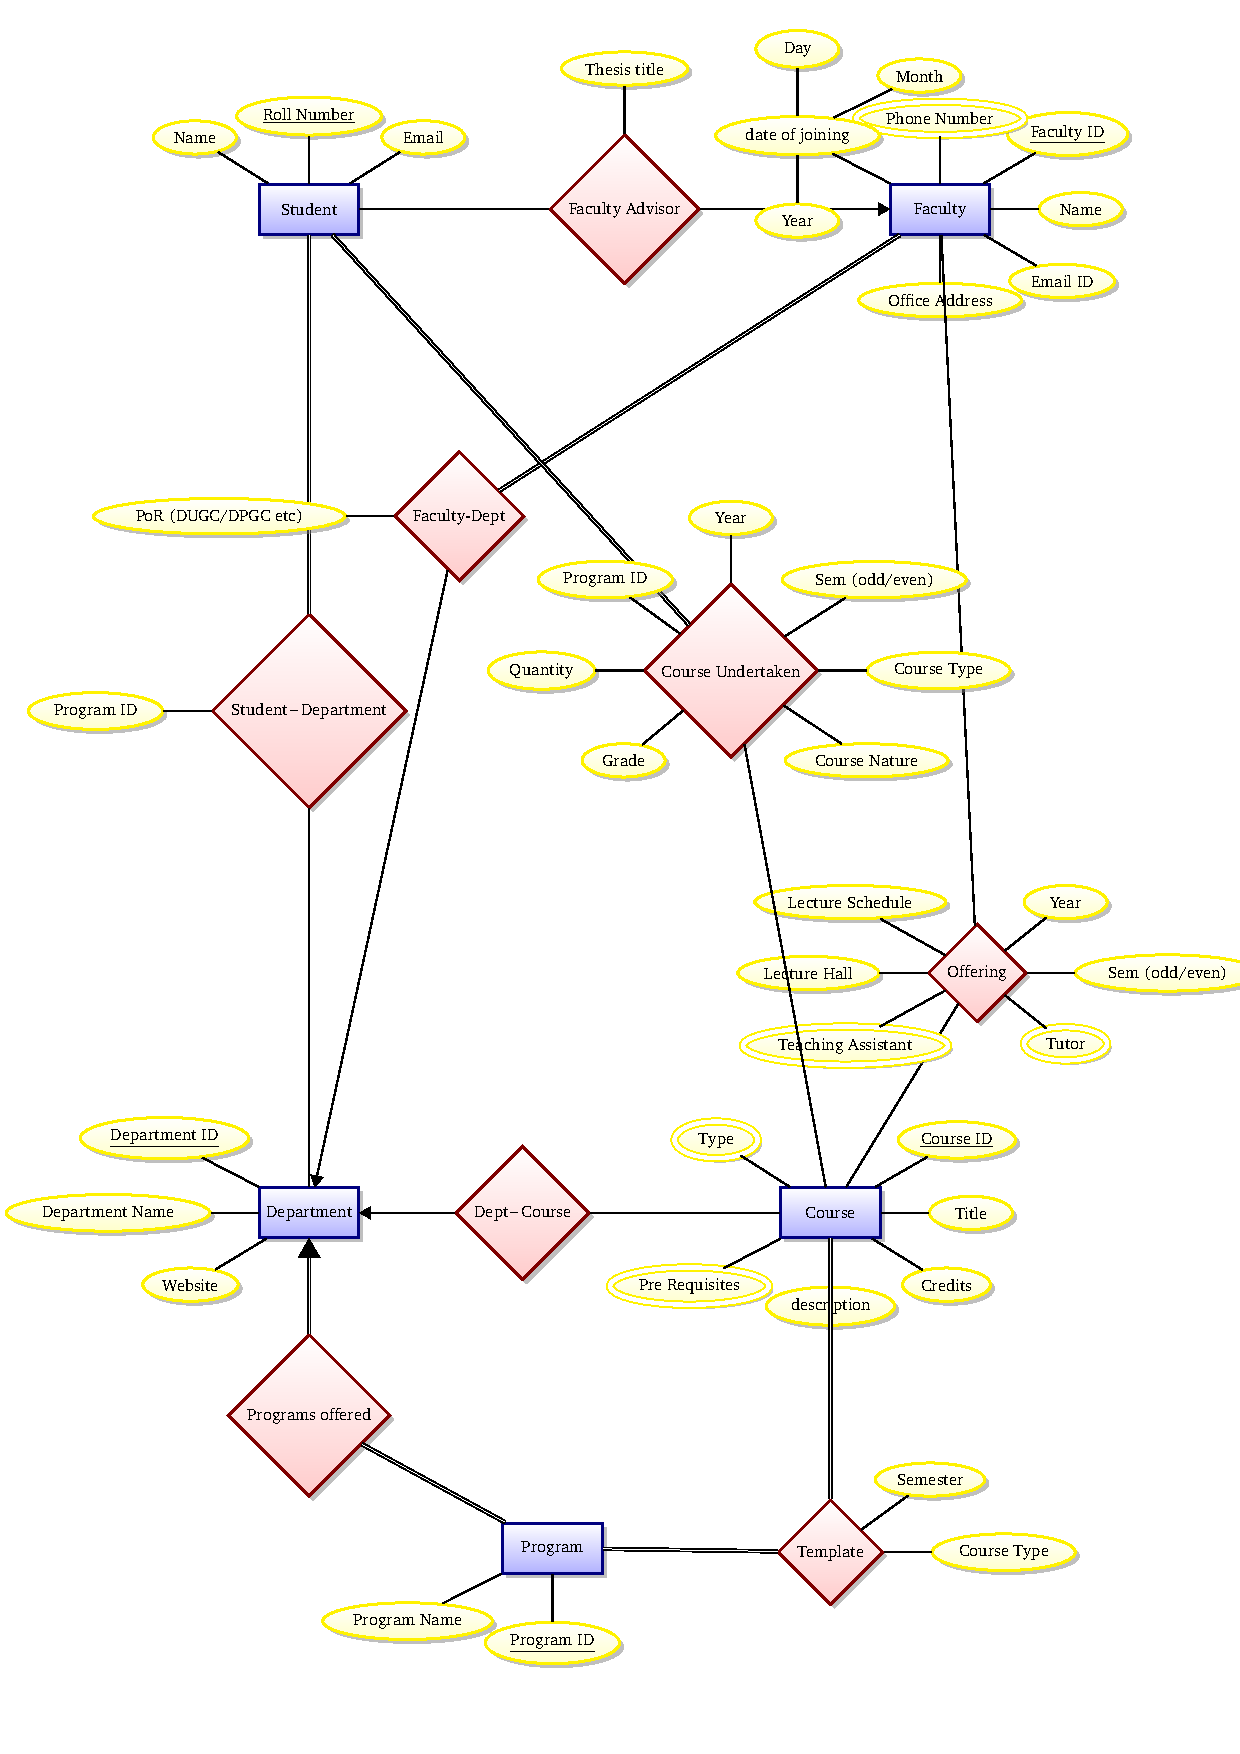
\includepdf[page={1}]{model.pdf}
\section*{Entity Relation Model for Academic system of IITK}
Above ER Model descibes the academic system of IIT Kanpur, lets discuss each of the attributes and relationships in more detail.

\subsection*{Entities}
\begin{itemize}
	\item{\textbf{Student:}} The student entity has a unique Roll Number, with other attributes being name, emailID.
	We can derive other things like the batch of student, year of joining from the roll number.
	\item{\textbf{Faculty:}} Faculty has a unique code (faculty ID) which acts as the primary key.
	Faculty entity also has office address, phone number/s etc.
	\item{\textbf{Department:}} Department entity has a unique department ID, website and the name.
	We can store other things like department addess etc, but that won't be relevant for academic prespective.
	\item{\textbf{Course:}} This entity represent the courses available in IITK, with couse ID being the primary key.
	Courses have a mutli valued attribute type, which represent the different caregories in which
	this course can be taken, for eg DE, OE, HSS etc. Note that pre requisites is also a multi valued attribute,
	since there can be more  than one pre-reqs.
	\item{\textbf{Program:}} This entity represent the different programs offered in a particular department.
	This can be BTech, MTech, PhD or minor in Algorithms etc. This entity is uniquely identified by the program ID.
\end{itemize}


\subsection*{Relationships}
\begin{itemize}
	\item{\textbf{Faculty Advisor:}} This relationship is useful for MTech/PhD students, it represents
	the faculty advisor for that student. Attribute thesis title is needed for research title.
	Note that we can also store the UGP supervisors for the UG students here.
	\item{\textbf{Student-Department:}} This relationship define how a student is related to a particular department.
	It has attribute program ID to represent this relation. For example student A is doing minors in
	Algorithms, then he is related to CSE with program ID = program\_ID(algorithms).
	\item{\textbf{Faculty-Dept:}} It represents the department which a facult belongs to. 
	It has a attribute PoR to represent if he is holding some position in the academic committee of department,
	eg Prof. Anil Seth is DUGC of CSE, so this attribute will be DUGC for him.
	\item{\textbf{Course Undertaken:}} This relationship is to define the courses a student has done
	in past or doing currently. It has attribute grade, which can be used in SPI/CPI calculation.\\
	Course Nature is fresh/repeat etc. Course type is used to represent how this student is doing this course,
	as student A might do CS315 as DE, while other might do it as an OE.\\
	Program ID is maintained to know this student is doing this course in order to complete which program.
	For example student A might be doing ESO207 in order to complete his BTech in CSE, while B might do
	ESO207 to complete a minor in algorithms. \\
	Quantity attribute is used to encorporate thesis course. for normal course this value is $1$.
	But for MTech/PhD this can be $>1$. Lets say that student A is taking $4$ thesis credits, this would mean
	that he is taking course CS699 (or other equivalant) $4$ times, for which he would get diffent grades. \\
	Also note that grade is a mutli valued attribute for the above reason, as an MTech might get 3 diffent
	grades in the 3 thesis credits.
	\item{\textbf{Offering:}} This relationship between course and faculty reprents the offering of this
	course by this particular faculty. This offering has year, semester as attribute as a instructor might
	offer same course multiple times. This relationship also contain some other relevant informations like lecture hall,
	tutors, TA, and course timings.
	\item{\textbf{Dept-Course:}} This relationship is necessary since a course is offered by faculty members
	of a particular department only. For example MTH101, would only be offered by faculty members of mathematics department only.

	\item{\textbf{Programs offered}} This relationship incorporates which all programs are offered by a
	particular department. For example CSE offers minors in 5-6 fields, major, BTech, Dual etc.
	\item{\textbf{Template}} Relationship between program and course is needed to store which all course one
	needs to complete in order to get this program's recognition. This relationship has an attribute semester,
	which would signify, in which semester one should do this course, for example, CSE BTechs need to do LIF101
	in $2^{nd}$ semester. Course type is similar to what we discussed in course entity. ie how one should take this
	course in order to complete the template. For eg LIF101 should be done as IC by UGs.
\end{itemize}

\end{document}